\scanpage{60}

Idem pour $A_*$ muni d'une structure \unsure{suppl.} --- p.ex. de groupe abélien, éventuellement diff et gradué. Dans ce dernier cas --- si les degrés sont bornés \unsure{infér\textsuperscript{t}} --- on peut donc prendre l'hypercohomologie
\[
\mathbb R^*\Gamma_{\unsure{?}}(X,A_*^*)
\overset{\mathrm{dfn}}{=}
\mathbb R^*\Gamma_X(\uline{A_{*X}^*})
\]
\margin{complexe induit par $A_*^*$ sur $X$ ou $A_*^*\times X/X$}

\figure{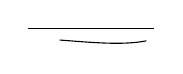
\begin{tikzpicture}
\draw (0,0)--(1.6,0);
\draw (.4,-.15).. controls (.8,-.18) and (1.2,-.22)..(1.5,-.16);
\end{tikzpicture}}

Soit $A$\inserted{$:(\unsure{\Delta}/X)^\circ\longrightarrow(\mathrm{Ab})$} un groupe sur $X$, considérons le complexe des cochaines sur $X$ à coeff. ds $A$
\[
C^{\unsure{n}}(X,A)\overset{\mathrm{dfn}}{=}
\prod_{\substack{\sigma\in\operatorname{Ob}\Delta_n/X\\=X_n}}A(\sigma)\quad,
\]
Les $C^n$ forment un groupe co $\frac12$ simplicial

\margin{59}
